%\documentclass[manusscript, 12p, authoryear]{elsarticle}
%\usepackage{setspace}
%\usepackage{geometry}                % See geometry.pdf to learn the layout options. There are lots.
%\geometry{letterpaper}                   % ... or a4paper or a5paper or ... 
%%\geometry{landscape}                % Activate for for rotated page geometry
%%\usepackage[parfill]{parskip}    % Activate to begin paragraphs with an empty line rather than an indent
%%% The lineno packages adds line numbers. Start line numbering with
%%% \begin{linenumbers}, end it with \end{linenumbers}. Or switch it on
%%% for the whole article with \linenumbers after \end{frontmatter}.
%\setlength{\parindent}{0in}
%\usepackage{graphicx}
%\usepackage{amsmath}
%\usepackage{amssymb}
%\usepackage{siunitx}
%\usepackage{textcomp}
%\usepackage{epstopdf}
%%\usepackage{lineno}
%\DeclareGraphicsRule{.tif}{png}{.png}{`convert #1 `dirname #1`/`basename #1 .tif`.png}
%\usepackage{color}
%\usepackage{url}
%\usepackage{wasysym}
%%comments
%\usepackage{color}
%\newcommand{\MWComment}[1]{{\small\color{green} #1}}
%\newcommand{\TFComment}[1]{{\small\color{blue} #1}}
%\newcommand{\JBComment}[1]{{\small\color{red} #1}}
%\newcommand{\NDComment}[1]{{\small\color{orange} #1}}
%
%\title{Supplementary Material\\The MANgrove-GroundwAter feedback model (MANGA) \\ ODD - Protocol}
%
%
%\author[1,2]{Jasper Bathmann\corref{cor1}%
%}
%\ead{Jasper.Bathmann@ufz.de}
%\author[3]{Ronny Peters}
%\author[1]{Dmitri Naumov}
%\author[1]{Thomas Fischer}
%\author[3]{Uta Berger}
%\author[1,2]{Marc Walther}
%
%\cortext[cor1]{Corresponding author: Jasper.Bathmann@ufz.de}
%
%\address[1]{Department of Environmental Informatics, UFZ, Permoserstra\ss e 15, 04318 Leipzig, Germany}
%\address[2]{Institute for Groundwater Management, Technische Universit\"at Dresden, 01069 Dresden, Germany}
%\address[3]{Institute of Forest Growth and Forest Computer Sciences, Technische Universit\"at Dresden, 01069 Dresden, Germany}
%
%\journal{Ecological Modelling}
%\date{January 2019}                                           % Activate to display a given date or no date
In the following chapter, the ODD for the MANGA model is presented.
Motivation and general derivation of the model are provided in the course of this thesis, but this chapter is following the standard protocol for code documentation in individual-based models \citep{Grimm2020}.


    \section{Bibliographic Information}
    % The package biblatex which supports \fullcite collides with the package multibbl
    % I have not found a solution how to print a bib item in the text so I write it out.
    % If you find a solution, please, post it here: https://tex.stackexchange.com/questions/173935
%
%
%\bibentry{Fischer2019}
\textbf{BIBENTRY FEHLT!}
    
\section{Author's contribution}
%\author[1]{Thomas Fischer}
%\author[1,2]{Jasper Bathmann}
%\author[1]{Dmitri Naumov}
%\author[1,3]{Fabien Magri}
%\author[1,2]{Marc Walther}
%\author[1,2]{Olaf Kolditz}
The author JB contributed to all parts of the protocol presented below.
The author drafted the text and derived the equation system of the groundwater flow model and coordinated the revision and editing process with the co-authors. Furthermore, the author implemented the presented model and coordinated further joint code developments, version control and code review processes.
    
    \section{Copyright Notice}
    
    \textbf{DOI FEHL!}
    \copyright 2020 Elsevier B.V. 
    
    The following is an near verbatim version of the supplementary materials of the accepted article published in Agricultural and Forest Meteorology (\href{https://doi.org/10.1016/j.ecolmodel.2020.108973}{doi:10.1016/j.ecolmodel.2020.108973}). The publisher ELSEVIER grants the Author the right to ``Include [the article] in a thesis or dissertation (provided this is not published commercially)'' \footnote{\href{https://www.elsevier.com/about/policies/copyright}{https://www.elsevier.com/about/policies/copyright; last accessed 20.04.2021}}.    
    \clearpage
    


\section{The pyMANGA ODD }
This chapter is a standard ODD protocol for agent-based model documentation following the description in \citet{Grimm2020}.
\subsection{Overview}
\subsubsection{Purpose and Patterns}
Characteristic mangrove growth form structures and species zonation patterns along transects in the intertidal zone are observed. 
To study how those patterns depend on groundwater salinity, MANGA is introduced.
It is an agent-based mangrove stand dynamics model which couples the single-tree model BETTINA \citep{Ronny2014} for tree growth dynamics and the subsurface hydrodynamic model OpenGeoSys (www.opengeosys.org).
The purpose of the coupled model is to analyze and understand the two-way feedback between porewater salinity and tree (fresh-)water use.
From abiotic boundary conditions like groundwater gradients and salt dilution by tidal water, emerge vegetation patterns like zonation of species composition or allometric manifestation of the trees (i.e.~dwarfing).
In particular, the effects of different hydraulic properties of the sediment, groundwater flow velocities and tidal affected ground water (re-)composition can be studied.
Additionally, the spatial and temporal groundwater salinity distribution can be observed.



\subsection{Entities, state variables and scales}
The MANGA model is using two already existing models as components.
The process variables and scales can be classified in two distinct levels.

The biotic tree population is simulated with a set of individual trees represented by the mangrove model BETTINA \citep{Ronny2014}.
This level is denoted \textit{flora} in the following.
Porewater salinity dynamics are calculated with OpenGeoSys (www.opengeosys.org).
\textit{Land} is the name for this level.

The two levels differ in time stepping and spatial scales as well as in their state variables and will be described in detail below.
\subsubsection{Flora}
The \textit{flora} consists of individual trees - the entities which are used as agents.
Every entity within the population is described by its static position ($x$, $y$), static species, dynamic age and dynamic allometry.
Allometry information includes stem radius, stem height, root radius and crown radius.
The full set of state variables defining the individual tree is listed in table \ref{tab_bettina_variables}.
Typical sizes of individuals are in the range of meters, whereas the whole \textit{flora} can be positioned within continuous spatial scales ranging from $\mathrm{m^2}$ to $\mathrm{km^2}$, such that mangrove stand dynamics can be studied.
The \textit{flora} dynamics are simulated in time-steps in the range from days up to one year.
Within this time stepping, tree growth dynamics is satisfyingly resolved.
\begin{table}[h]
\centering
\begin{tabular}{|c|c|c|}
\hline 
\multicolumn{2}{|c|}{Variable} & Typical Scale \\
Symbol & Denotation & \\ 
\hline 
$r_S$ & stem radius  & \SIrange{0.01}{1.0}{m}  \\ 
\hline 
$h_S$ & stem height  & \SIrange{0.1}{10.0}{m}  \\ 
\hline 
$r_R$ & root radius  & \SIrange{0.1}{10.0}{m}  \\ 
\hline 
$r_C$ & crown radius  & \SIrange{0.1}{10.0}{m}  \\ 
\hline 
$t_T$ & tree age  & \SIrange{0.1}{10.0}{m} \\ 
\hline 
$\vec{r}$ & tree position  &   \\ 
\hline 
\end{tabular} 
\caption{State variables of individual trees.
All listed variables are floating point numbers.}\label{tab_bettina_variables}
\end{table}
\subsubsection{Land}
The \textit{land} is representing the soil on which trees grow.
Two scalar variables, porewater salinity and hydrostatic pressure, are defined on a three dimensional abiotic aquifer system and one 3 dimensional vector field of secondary variables represents the Darcy velocity.
Considered aquifer depths are in the range of $\mathrm{m}$, corresponding to the depth of subsurface layers with relatively high water permeability.
The horizontal system extension can range from $\mathrm{m^2}$ to $\mathrm{km^2}$ but must be larger or equal than the \textit{flora} extension in order to allow to study tree population dynamics.
The abiotic processes are simulated on timescales ranging from \SI{1e-2}{s} to \SI{1e5}{s} depending on the rate of change in variables.

\subsection{Process Overview and Scheduling}
\subsubsection{Model Components} 
Two independent models, BETTINA for \textit{flora} and OpenGeoSys for \textit{land}, are coupled.
The information of state variables and parameters of \textit{flora} is passed to OpenGeoSys with the time stepping from the \textit{flora} model.
The \textit{land} model uses this information to dynamically update the \textit{flora's} influence on the abiotic processes, namely fresh water flow from the aquifer into the plants (i.e.~plant water uptake).
The water uptake is controlled by the osmotic potential, and thereby by porewater salinity.
Porewater salinity is one of the two variables for the hydrodynamic model OpenGeoSys.

The OpenGeoSys software to uses a finer time stepping on scales, where state variables of the \textit{flora} can be regarded as constant.
After solving the abiotic processes, the updated information of current porewater salinity distribution in high temporal resolution is passed to BETTINA which uses the information on average available resources to update the \textit{flora}.
The new \textit{flora} state is passed back to OpenGeoSys.
Consequently, long time simulations are performed using the iteration over the subsequent cycle of
\begin{enumerate}
\item BETTINA update and
\item OpenGeoSys calculations.

\end{enumerate}

\subsubsection{Flora}
Dynamics on the \textit{flora} level are described by four sub-models.
A sketch of BETTINA inherent plant dynamics is given in Figure \ref{fig_bettina_sketch}.
\begin{figure}[h]\centering
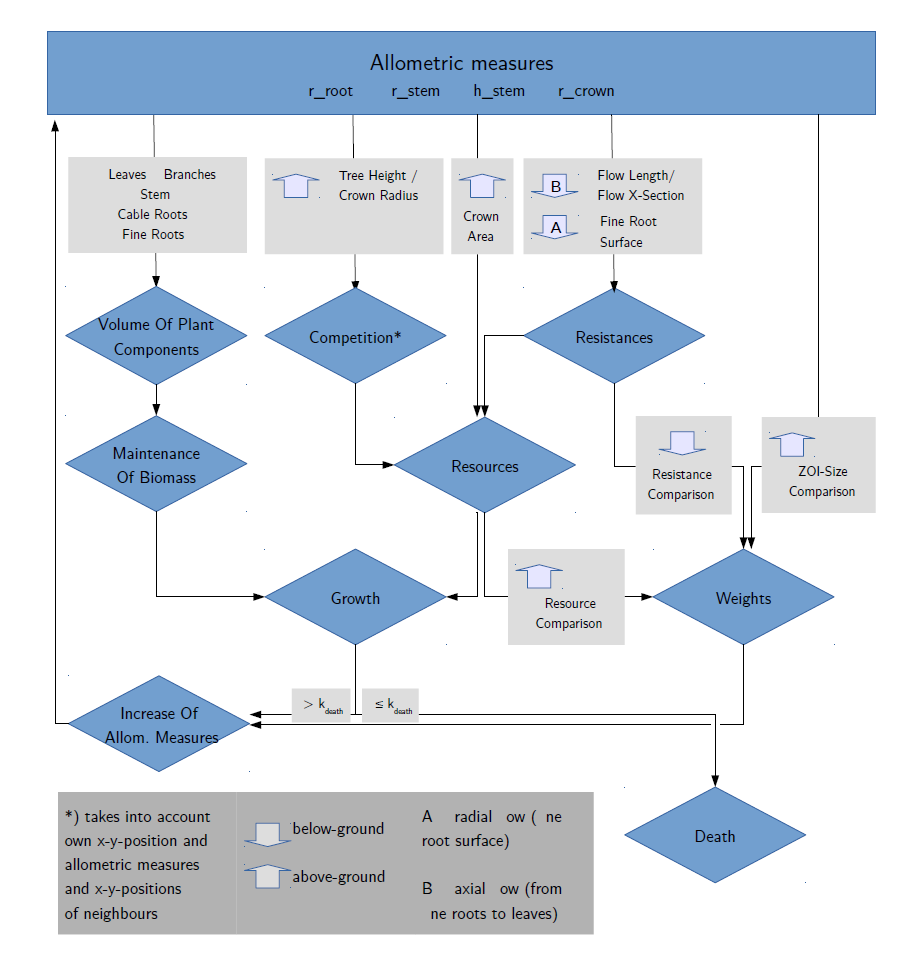
\includegraphics[width=.8\textwidth]{ODD_MANGA/bettina_sketch.png} 
\caption{Sketch of iteration cycle for \textit{flora} dynamics modelled with BETTINA. Illustration is adapted from \citet{Ronny2014}--(supplementary material).}\label{fig_bettina_sketch}
\end{figure} 

The first sub-model ("Competition" in fig. 1) predicts the penalty of aboveground competition on light interception using a modified \textbf{Z}one \textbf{o}f \textbf{I}nfluence (ZOI, \citet{Gates1978}) approach with complete asymmetric competition \citep{Schwinning1998}.
The second sub-model ("Resistances" and "Resources" in fig. 1) simulates the above- and belowground resource uptake of individual trees and depends on the calculated shading penalties, porewater salinity and tree allometry.
Subsequently, depending on the current tree volume, the third sub-model ("Volume of Plant Components" and "Maintenance of Biomass" in fig. 1) calculates how much resources are required for tree maintenance.
The surplus of available resources determines the amount of resources available for tree growth ("Growth" in fig. 1). 
Finally, the fourth sub-model ("Increase of Allometric Measures" in fig. 1) distributes tree growth to an increase of the allometric measures, e.g. it updates the tree's state variables.
The growth is distributed according to maintain a constant proportion of light and water availability ("Weights" in fig. 1).
If resources for growth are negative (i.e., the amount of resource demanded for tree maintenance exceeds the resource availability), trees eventually die ("Death" in fig. 1).
At each time step all four sub models are applied in a sequence (see sub-models part for details): 
\begin{enumerate}
\item aboveground competition
\item resource uptake
\item biomass maintenance and resources for growth
\item tree growth and death
\end{enumerate}
Beside the porewater salinity distribution, the sub-models depend on species-specific parameters such as minimal leaf water potential, sap flow conductivity (xylem conductivity), fine root permeability, a geometrical factor for fine root surface per area of root extension, maintenance factor, ratio of available resources used for production of new biomass, and photosynthesis energy efficiency (light-water-ratio), and three factors describing the tendency for equilibria in (i) resource uptake, (ii) flow resistances and (iii) tree crown and root disk size.
Those parameters will be explained in detail in the sub-model section.
\subsubsection{Land}
The abiotic subsurface processes are described by solving a system of PDEs on a grid with OpenGeoSys (www.opengeosys.org).
The equations describing the system dynamics consist of one equation describing the total groundwater mass flow and one describing the subsurface salinity mass flow.

System boundary conditions, temporal resolution and the method to solve the equations are also provided within project files.
The tree entities provide additional source terms in the root zone, which depend on state variables and parameters of the \textit{flora}, controlling the water uptake of the trees (see belowground resource uptake).
\subsection{Design Concepts}
\subsubsection{Basic Principles}
In tree dynamics described on the \textit{flora} level, the considered resources are restricted to light (above-ground) and water (below-ground).
The model describes resource uptake and growth mechanistically.
The resource uptake depends on the allometric measures of the plant.
Light interception is proportional to crown area.
Water uptake is described with Darcy’s law.
According to the assumptions of the pipe-model theory (Rennolls, 1994), the characteristics of the vertical flow path is homogeneous along the flow axis.

Further basic assumptions for the tree model are:
\begin{itemize}
\item Proportional use of above- and below-ground resources.
\item Maintenance costs are proportional to the total biomass.
\item Resources for plant growth are the difference between available resources and maintenance cost.
\item Allometric allocation of resources during growth is performed to improve resource uptake at the individual bottleneck of each plant.
\end{itemize}
For the subsurface salinity dynamics on the \textit{land} level mass- and momentum conservation are considered.
Additionally, phenomenological laws of Fickian type dispersive mass flux, the Bear-Scheidegger dispersion relationship and Newtons viscosity law are used.
Further, porewater density is regarded as a function of pressure and porewater salinity only.
The porewater is taken as incompressible with constant dynamic viscosity.
The interfacial drag term of momentum exchange is approximated up to the 2nd order in bulk flow velocity.
Within the momentum balance, inertia is neglected and forces are regarded up to linear order in bulk velocity.
\subsubsection{Emergence}
The features at the plant population level, i.e.~zonation patterns regarding species distribution and tree allometry, mortality and maximum tree height, emerge from the individual growth and death.
These features are influenced by resource availability due to the spatial temporal groundwater salinity redistribution and competition for sunlight with neighbors.\\
On the \textit{land} level in turn, groundwater salinity distributions are emerging from the model.
It is influenced by the plant distribution and abiotic parameters such as hydraulic conductivity and aquifer depth.
\subsubsection{Adaption}
Individual trees adapt to environmental conditions by growth allocation, in order to optimize resource uptake.
For example, a tree with a canopy shadowed by other trees, allocates most of its resources into growth of crown radius and stem height.
\subsubsection{Objectives}
Trees follow no objectives apart from individual growth under the constraint of maximized resource uptake.
\subsubsection{Learning}
Learning of agents is not implemented.
However, individual trees adapt to environmental conditions (see adaption).
\subsubsection{Prediction}
Prediction of future conditions by individuals is not implemented.
\subsubsection{Sensing}
Individuals within the \textit{flora} get information on the locally available resources.

Resource availability is results from the interactions and competition within the local neighborhood and the porewater salinity distribution.
\subsubsection{Interaction}
Individual trees compete for sunlight.
This competition is described in a simplified manner using a modified ZOI competition concept. 
Competition is assumed to be completely asymmetric.
Competition strength is determined by tree height and the size of the ZOI is given by the crown radius.
At locations, where a tree is the highest, this individual takes all available energy.

Competition for belowground resources is emerging from the subsurface flow and dilution processes.
\subsubsection{Stochasticity}
Within the MANGA model, stochasticity is limited to the initial seedling distribution and positioning of new seedlings (recruitment).

Further stochasticity can be incorporated by stochastic boundary conditions, e.g. the representation of rarely occurring extreme weather events such as hurricanes.
\subsubsection{Collectives}
Tree entities can be arbitrarily grouped in any kind of collective at the stage of model initialization. 
However, each tree group can be associated to a sub-domain of the model area, where it is allowed to grow.
Additionally, for each tree group, a specific species can be attributed which is represented by species-specific model parameters.
\subsubsection{Observation}
The MANGA model allows to continuously register all state variables listed above.
Typically, \textit{flora} state variables such as tree position, information on tree allometry and tree age are monitored at each BETTINA time step.
The porewater salinity can be monitored with arbitrarily fine temporal resolution.
All output files can be visualized and analyzed externally.

\subsection*{Details}
\subsection{Initialization}

\begin{enumerate}
\item Established trees have set initial allometric measures and species-specific parameters.
Additionally, arbitrary (random, rows, ...) initial plant distribution can be chosen.
\item On the \textit{land} level, OpenGeoSys is initialized by a set of abiotic parameter fields combined with initial- and boundary conditions.
\end{enumerate}

\subsection{Input}
External perturbations to the abiotic dynamics such as tidal flooding or sea level rise or extreme weather events can be accounted for by means of time dependent boundary conditions.
Additionally, perturbations to the biosphere can be defined (logging, fire). 
\subsection{Submodels}
\subsubsection{Model Components}
Key innovation of MANGA is the dynamic coupling of the two independent models OpenGeoSys and BETTINA.
On the one hand, information of the \textit{flora} is passed to the abiotic processes by means of boundary conditions defined in the tree root regions.
On the other hand, the \textit{flora} dynamics are directly influenced by the dynamic porewater salinity distribution, which is passed to BETTINA from the OpenGeoSys output.\\
BETTINA and OpenGeoSys are implemented as modules to the MANGA model.
Hence, both modules can be used independently or replaced readily.
The modular coupling scheme is sketched in \citet{Bathmann2020}.


\subsubsection{Flora}
The individual growth of the plant and the distribution onto the different plant components is the heart of BETTINA.
In general, tree growth has a deterministic description and depends on the tree allometry, tree environment and the available resources.

Detailed information on competition for resources, resource uptake, tree maintenance, resource availability and tree growth is provided below and derived from \citet{Ronny2014} and \citet{Peters2018}.
Parameters used to parameterize BETTINA are listed in table \ref{tab_bettina_parameter} and explained in detail in \citet{Ronny2014}.
\paragraph{\textbf{Belowground Competition}}
Belowground competition emerges automatically from the MANGA coupling of \textit{land} and \textit{flora} objects.
\paragraph{\textbf{Aboveground Competition}}
The submodel for aboveground competition accounts for the interactions between the trees and considers the spatial location of agents.
Shadowing coefficients for every tree are calculated using the following scheme:
\begin{enumerate}
\item set the tree-owned variable $N^{\text{taller}}_i$ to the number of trees being higher at a mesh node $i$ within the crown radius.
\item calculate the shadowing coefficient $C_S\in [0,1]$ for the whole crown
\begin{equation}
C_S = 1-\frac{\sum_i 0^{N^{\text{taller}}_i} A_i}{\sum_i A_i},
\end{equation}
with $A_i$ being the fraction of crown area associated to mesh node $i$.
\end{enumerate}
\paragraph{\textbf{Resource Uptake}}
For resource uptake, Darcy's law for laminar flow is applied to calculate maximum (fresh-)water flow $Q$ from the roots to the canopy
\begin{align}
Q = -\frac{\Psi_{\text{leaf}}- \Psi_{\text{h}} -\Psi_{\text{osmo}}}{R_1 + R_2}
\end{align}
with hydrostatic potential gradient $\Delta \Psi$ and flow resistances $R_i$.
The hydrostatic potential consists of the minimal leaf potential $\Psi_{\text{leaf}}$ (species-specific parameter), the osmotic potential 
\begin{align}
\Psi_{\text{osmo}}= -\SI{85000}{\frac{m^2}{s}}S,
\end{align}
with porewater salinity $S(t)$ and the height potential 
\begin{align}
\Psi_h = \rho_R g (2r_C+h_S).
\end{align}
The resistance $R = R_1+R_2$ consists of
\begin{align}
R_1 &= \frac{1}{L_p k_g \pi r_R^2 h_R} ,\end{align}
with root thickness $h_r$, species-specific root surface permeability $L_p$ and geometrical factor $k_g$.
The equation represents the flow resistance through the fine roots and 
\begin{align}
R_2 &= \frac{l_{\text{flow}}}{k_f \pi r_S^2}.
\end{align}
representing the resistance along the flow path through the trees cable roots, stem and branches (with species-specific xylem conductivity $k_f$).
The flow length $l_{\text{flow}}$ reads,
\begin{align}
l_{\text{flow}} = 2 r_c + h_c + \sqrt{\frac{1}{2}} r_r
\end{align}
Both resistances depend on the current tree allometry.

Integration of mass flow $Q$ from start time $t_1$ of the current time step to its final time $t_2$ normalized to the daily cycle provides the total uptake of belowground resources for each tree during the time step:
\begin{align}
RES_B = \int_{t_1}^{t_2} \frac{Q}{\pi} \mathrm{d}t.
\end{align}
Without the sinusoidal pattern daily transpiration values are overestimated. Since we want to estimate a realistic feedback on porewater, we included an improved quantification of daily water fluxes \citep{Peters2020}.
Calculation of available aboveground resources reads
\begin{align}
RES_A = \int_{t_1}^{t_2} (1-C_S) S_e R_S \pi r_C^2 \mathrm{d}t,
\end{align}
with the calculated shadowing coefficient $C_S$, solar photosynthesis energy efficiency ($S_e$ and solar constant $R_S$.
Finally, the total available resources are either limited by solar energy or by available fresh water:
\begin{align}
RES_{\text{available}} = \text{min}\left(RES_A, RES_B\right).
\end{align}
\paragraph{\textbf{Tree maintenance and growth resource availability}}
A portion of resources is assumed to be consumed by tree maintenance, which is proportional to the tree volume.
Available resources for tree growth
\begin{align}
RES_{\text{growth}} = RES_{\text{available}} - k_m V_{\text{tree}}
\end{align}
depend on the difference of available resources and maintenance cost.
Maintenance factor $k_m$ denotes the species-specific maintenance cost per tree volume $V_{\text{tree}}$.
\paragraph{\textbf{Growth and Death}}
All individual trees for which the resources available for growth are smaller than a species-specific death level $k_{grow}$, meaning
\begin{align}
k_{grow} > RES_{\text{growth}},
\end{align}
die and do not longer persist in the model.
Surviving trees allocate the resources available for growth in order to optimize resource uptake.

\textit{Growth weights}
are set to distribute growth mainly in the way to predominately increase specific allometric measures for improving resource uptake at the bottleneck.
To define, how strong a mechanism shall be promoted, first some standardized growth weights are calculated
\begin{enumerate}
\item to quantify, whether the tree lacks either above- or below-ground resources,
$q_{res}$ is set as the ratio
$\frac{RES_A - RES_B}{RES_A + RES_B}$ and 
\item to quantify, which of the resistances limits water flow, $q_r$ is set as the ratio $\frac{R_1 - R_2}{R_1 + R_2}$.
\item Stem height growth is intended to give advantage for above-ground competition.
Assuming, if the crown radius is bigger than the root radius, above-ground competition is expected to be stronger, we set $q_{rad}$ as the ratio $\frac{r_c - r_r}{r_c + r_r}$.
\end{enumerate}
With these auxiliary variables, the growth weights are estimated by means of sigmoidal estimators as
\begin{itemize}
\item the weight for increasing stem height $h_s$ as 
$\omega_h = \frac{1}{1 + \exp\left(-\frac{q_{rad}}{\sigma_2}\right)}$,
\item the weight for increasing crown radius $r_c$ as 
$\omega_c = \frac{1 - \omega_h}{1 + \exp\left(-\frac{q_{res}}{\sigma_1}\right)}$,
\item the weight for increasing stem radius $r_s$ as 
$\omega_s = \frac{1 - \omega_h-\omega_c}{1 + \exp\left(-\frac{q_r}{\sigma_1}\right)}$, and
\item the weight for increasing root radius $r_r$ as 
$\omega_r = 1 - \omega_h-\omega_c - \omega_s$.
\end{itemize}
\textbf{Growth} is performed using the remaining resources for a specific increase of biomass (volume).
The allometric relations allow for a calculation (derivation in \citet{Ronny2014}) of the increase in respective measures which follows as increment of
\begin{itemize}
\item stem height $\Delta h_s = \frac{\omega_h }{\pi^2 r_s^2}\cdot RES_{\text{growth}}$,
\item stem radius $\Delta r_s = \frac{\omega_s}{2\pi r_s l_f}\cdot RES_{\text{growth}}$,
\item crown radius $\Delta r_c = \frac{\omega_c }{2\pi \left(r_c h_c + r_s^2\right)}\cdot RES_{\text{growth}}$ and
\item root radius $\Delta r_r = \frac{\omega_r}{2 \pi r_r h_r + \pi \frac{r_s^2}{\sqrt{2}}}\cdot RES_{\text{growth}}$.
\end{itemize}

%- the crown radius rcrown increases by
%wa1 · growth
%2 · π · (rcrown · hcrown + rstem
%)
% 2
%- the root radius rroot increases by
%wb1 · growth
%2 · π · rroot · hroot + 2−0.5 · π · rstem
% 2
%- the stem radius rstem increases by
%wb2 · growth
%2 · π · rstem · (2 · rcrown + hstem + 2−0.5 · rroot
% 2
% )
%
%


\begin{table}[h]
\centering
\begin{tabular}{|c|c|c|c|}
Symbol & {Parameter Name} &{Typical Value} \\ 

%Symbol & Denotation & \textit{Avicennia germinans}  \\ 
\hline\hline 
$R_{s}$ & solar constant  & \SI{5e-8}{kg/s/m^2} \\ 
\hline 
$h_R^i$ & root depth (constant) & \SI{4e-3}{m} \\ 
\hline 
$h_C$ & leaf canopy thickness (constant) & \SI{4e-3}{m} \\ 
\hline 
$r_R^i$ & initial root radius & \SI{0.25}{m} \\ 
\hline 
$r_S^i$ & initial stem radius & \SI{1e-2}{m} \\ 
\hline 
$h_S^i$ & initial stem height & \SI{1.5e-2}{m} \\ 
\hline 
$r_C^i$ & initial crown radius & \SI{0.3}{m} \\ 
\hline 
$\Psi_{\text{leaf}}$ & minimum leaf water potential & \SI{-8.15}{MPa}  \\ 
\hline 
$k_f$ & xylem conductivity & \SI{3.3e-15}{kg/s/m^2} \\ 
\hline 
$L_p$ & fine root permeability & \SI{1e-10}{m^2} \\ 
\hline 
$k_g$ & geometrical factor & $4000$  \\ 
\hline 
$\omega_{1}$ & growth weight one & $0.0035$ \\ 
\hline 
$\sigma_{1}$ & weight function slope 1 & 0.05\\ 
\hline 
$\sigma_{2}$ & weight function slope 2 & 0.015 \\ 
\hline 
$k_{\text{growth}}$ & maintenance factor & \SI{1.4e-6}{} \\ 
\hline 
\end{tabular} 
\caption{Parameters for the BETTINA module.}\label{tab_bettina_parameter}
\end{table}

\subsubsection{Land}
The assumption of saturated groundwater flow is made for the whole aquifer domain.

The abiotic subsurface processes are described by solving a system of PDEs on a grid. The equations describing the system dynamics consist of one equation describing the total groundwater mass flow 
\begin{equation}
\phi\frac{\partial  \rho_R}{\partial p}\frac{\partial p}{\partial t} + \phi\frac{\partial \rho_R}{\partial \omega_C}\frac{\partial \omega_C}{\partial t} - \nabla \left(\frac{\kappa}{\mu}\rho_R \left(\nabla p - \rho_R g \right)\right) + Q_p = 0,
\end{equation}
and one describing the groundwater salinity mass flow
\begin{equation}
\begin{split}
0 =&
\omega_C R\phi\frac{\partial  \rho_R }{\partial p}\frac{\partial p}{\partial t}+\omega_C R\phi\left(\frac{\rho_R}{\omega_C}+\frac{\partial  \rho_R }{\partial \omega_C}\right)\frac{\partial \omega_C}{\partial t} - \nabla \left(  \frac{\kappa}{\mu} \rho_R \omega_C \left(\nabla p - \rho_R g \right) + \rho_R \mathbf{D}_h \nabla \omega_C\right),
\end{split}
\end{equation}
with hydrostatic pressure $p$ and component concentration $\omega_C$. 
The parameters 
\begin{itemize}
\item density $\rho_R$,
\item permeability $\kappa$,
\item viscosity $\mu$,
\item gravitation constant $g$,
\item medium porosity $\Phi$,
\item retardation $R$, and
\item dispersion tensor $\mathbf{D}_h$
\end{itemize}
can be defined within external project files.
Typical orders of magnitude for the parameters used to model the abiotic processes are given in table \ref{tab_ogs_parameter}.
\paragraph{\textbf{Boundary Conditions in Tree Root Regions}}
The fresh water uptake of trees is given by freshwater sinks in the root region of individual trees.
The fresh water mass density flow reads
\begin{equation}
q_f = - \frac{\rho_R}{\pi r_R^2 r_D}\left(\frac{\Psi_{\text{leaf}} - \Psi_{\text{h}}-\Psi_{\text{osmo}}}{R_1+R_2}\right),
\end{equation}
Formulas for the resistances $R_1$ and $R_2$ as well as the individual potentials are given above.
The parameters for this boundary condition are directly taken from the last BETTINA time step.
\begin{table}[h] \label{tab_ogs_parameter}\centering
\begin{tabular}{|c|c|c|}
\hline 
\multicolumn{2}{|c|}{Parameter} & Typical Scale  \\ 
Symbol & Denotation & \\ 
\hline 
$\rho_R$ & fresh water density & $10^3 \frac{kg}{m^3}$ \\ 
\hline 
$\mu$ & dynamic viscosity & $10^{-3} \frac{kg}{ms}$ \\ 
\hline 
$\kappa$ & medium permeability & $(5...50)\cdot 10^{-12} m^2 \cdot{\text{diag}\left(1,1,1\right)}$ \\ 
\hline 
$\Phi$ & medium porosity & $0.5$ \\ 
\hline 
$D_m$ & molecular diffusion coefficient & $2\times 10^{-9} \frac{m^2}{s}$ \\ 
\hline 
$\beta_L$ & longitudinal solute dispersivity & $1m$ \\ 
\hline 
$\beta_T$ & transversal solute dispersivity & $0.2m$ \\  
\hline 
$g$ & gravitation constant & $9.81 \frac{1}{ms^2}$ \\  
\hline 
\end{tabular} 
\caption{Parameters for the OpenGeoSys module.}
\end{table}
%\bibliographystyle{apalike}
%\bibliography{bibtex.bib}
%\end{document}

